\newcommand{\holeexamplegraph}{
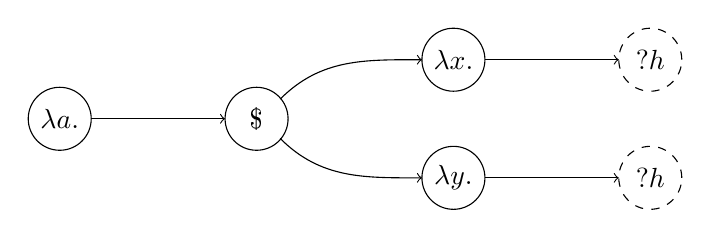
\begin{tikzpicture}

\draw (0,0)   circle (.4cm) node[align=center] {$\lambda a.$};
\draw (2.5,0) circle (.4cm) node[align=center] {\$};

\draw (5,.75) circle (.4cm) node[align=center] {$\lambda x.$};
\draw[dashed] (7.5,.75) circle (.4cm) node[align=center] {$?h$};

\draw (5,-.75) circle (.4cm) node[align=center] {$\lambda y.$};
\draw[dashed] (7.5,-.75) circle (.4cm) node[align=center] {$?h$};

\draw [->] (.4,0)     to [out=0,in=180]  (2.1,0);
\draw [->] (2.8,.25)  to [out=45,in=180] (4.6,.75);
\draw [->] (2.8,-.25) to [out=-45,in=180] (4.6,-.75);

\draw [->] (5.4,.75)  to [out=0,in=180] (7.1,.75);
\draw [->] (5.4,-.75) to [out=0,in=180] (7.1,-.75);

\end{tikzpicture}}

\newcommand{\cseexamplegraph}{
\begin{tikzpicture}
\draw (1.6,0)    circle (.4cm) node[align=center] {\$};

\draw (3.75,.75) circle (.4cm) node[align=center] {$\lambda x.$};
\draw (6.90,.75) node[draw,dashed,regular polygon, regular polygon sides=3, shape border rotate=90]
      {\phantom{b}$t$\phantom{g}};

\draw (3.75,-.75) circle (.4cm) node[align=center] {$\lambda a.$};
\draw (5.90,-.75) circle (.4cm) node[align=center] {$\lambda b.$};
\draw (9,-.75) node[draw,dashed,regular polygon, regular polygon sides=3, shape border rotate=90]
      {\phantom{b}$t$\phantom{g}};

\draw [->] (1.9,.27)  to [out=45,in=180] (3.35,.75);
\draw [->] (1.9,-.27) to [out=-45,in=180] (3.35,-.75);

\draw [->] (4.15,-.75) to [out=0,in=180]  (5.5,-.75);
\draw [->] (4.15,.75)  to [out=0,in=180]  (5.9,.75);

\draw [->] (6.3,-.75) to [out=0,in=180]  (8,-.75);

\end{tikzpicture}}

\newcommand{\codebruijnexamplegraph}{
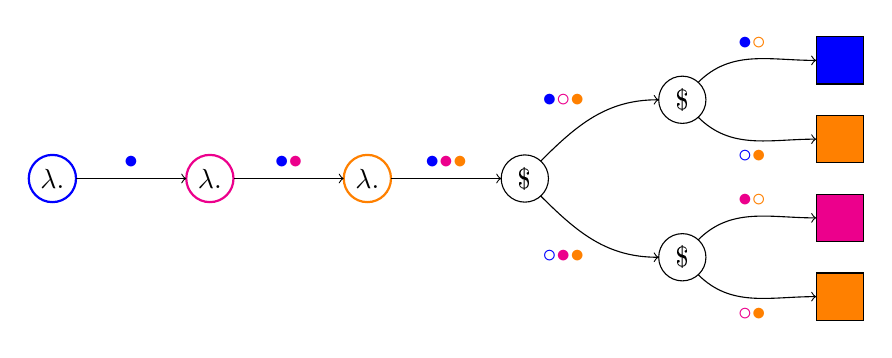
\begin{tikzpicture}
\draw[draw=blue   ,thick] (0,0) circle (.3cm) node[align=center] {$\lambda{}.$};
\draw[draw=magenta,thick] (2,0) circle (.3cm) node[align=center] {$\lambda{}.$};
\draw[draw=orange ,thick] (4,0) circle (.3cm) node[align=center] {$\lambda{}.$};

\draw (6,0) circle (.3cm) node[align=center] {\$};

\draw (8,1)    circle (.3cm) node[align=center] {\$};
\draw[fill=blue]   (10,1.5) +(-.3cm,-.3cm) rectangle +(.3cm,.3cm);
\draw[fill=orange] (10,.5)  +(-.3cm,-.3cm) rectangle +(.3cm,.3cm);

\draw (8,-1)    circle (.3cm) node[align=center] {\$};
\draw[fill=magenta] (10,-.5)  +(-.3cm,-.3cm) rectangle +(.3cm,.3cm);
\draw[fill=orange]  (10,-1.5) +(-.3cm,-.3cm) rectangle +(.3cm,.3cm);


\draw [->] (0.3,0)   to [out=0,in=180] node[above]{$\color{blue}{\bullet}$} (1.7,0);
\draw [->] (2.3,0)   to [out=0,in=180] node[above]{$\color{blue}{\bullet}\color{magenta}{\bullet}$} (3.7,0);
\draw [->] (4.3,0)   to [out=0,in=180] node[above]{$\color{blue}{\bullet}\color{magenta}{\bullet}\color{orange}{\bullet}$} (5.7,0);

\draw [->] (6.2,-.22)  to [out=-45,in=180] node[below left]{$\color{blue}{\circ}\color{magenta}{\bullet}\color{orange}{\bullet}$} (7.7,-1);
\draw [->] (6.2,.22)   to [out=45,in=180] node[above left]{$\color{blue}{\bullet}\color{magenta}{\circ}\color{orange}{\bullet}$} (7.7,1);
\draw [->] (8.2,1.22)  to [out=45,in=180] node[above]{$\color{blue}{\bullet}\color{orange}{\circ}$} (9.7,1.5);
\draw [->] (8.2,.78)   to [out=-45,in=180] node[below]{$\color{blue}{\circ}\color{orange}{\bullet}$} (9.7,.5);
\draw [->] (8.2,-.78)  to [out=45,in=180] node[above]{$\color{magenta}{\bullet}\color{orange}{\circ}$} (9.7,-.5);
\draw [->] (8.2,-1.22) to [out=-45,in=180] node[below]{$\color{magenta}{\circ}\color{orange}{\bullet}$} (9.7,-1.5);
\end{tikzpicture}
}
